\documentclass[aspectratio=169]{beamer}
\usepackage[utf8]{inputenc}
\usepackage[T1]{fontenc}
\usepackage{graphicx}
\usepackage{booktabs}
\usepackage{amsmath}
\usepackage{tikz}
\usetikzlibrary{positioning}
\usepackage{colortbl}
\usepackage{float}

% Theme
\usetheme{Madrid}
\usecolortheme{whale}

% Custom colors -- deep forest green palette
\definecolor{mycoDark}{RGB}{22, 72, 42}
\definecolor{mycoMid}{RGB}{46, 125, 50}
\definecolor{mycoLight}{RGB}{129, 199, 132}
\definecolor{mycoAccent}{RGB}{255, 167, 38}

\setbeamercolor{structure}{fg=mycoMid}
\setbeamercolor{palette primary}{bg=mycoDark,fg=white}
\setbeamercolor{palette secondary}{bg=mycoMid,fg=white}
\setbeamercolor{palette tertiary}{bg=mycoLight,fg=mycoDark}
\setbeamercolor{frametitle}{bg=mycoDark,fg=white}
\setbeamercolor{title}{fg=white,bg=mycoDark}
\setbeamercolor{block title}{bg=mycoDark,fg=white}
\setbeamercolor{block body}{bg=mycoDark!5,fg=black}
\setbeamercolor{alerted text}{fg=mycoAccent}
\setbeamercolor{itemize item}{fg=mycoMid}
\setbeamercolor{enumerate item}{fg=mycoMid}

\setbeamertemplate{navigation symbols}{}
\setbeamertemplate{footline}{
  \leavevmode%
  \hbox{%
  \begin{beamercolorbox}[wd=.7\paperwidth,ht=2.5ex,dp=1ex,left]{author in head/foot}%
    \hspace*{2ex}\insertshortauthor
  \end{beamercolorbox}%
  \begin{beamercolorbox}[wd=.3\paperwidth,ht=2.5ex,dp=1ex,right]{title in head/foot}%
    \insertframenumber{} / \inserttotalframenumber\hspace*{2ex}
  \end{beamercolorbox}}%
}

\graphicspath{{content/figures/}}

\title{MycoAI Retrieval}
\subtitle{Fungal Species Identification via Image Retrieval}
\author{Graduation Thesis}
\institute{MycoAI Lab -- HUST \& Utrecht}
\date{June 2025}

\begin{document}

% ===== SLIDE 1: TITLE =====
\begin{frame}
  \titlepage
\end{frame}

% ===== SLIDE 2: OUTLINE =====
\begin{frame}{Outline}
  \tableofcontents[hideallsubsections]
\end{frame}

% ===== SECTION: PREFACE =====
\section{Preface \& Motivation}

% ===== SLIDE 3: MOTIVATION =====
\begin{frame}{Why Fungi?}
  \begin{columns}[T]
    \begin{column}{0.55\textwidth}
      \textbf{The question:}
      \begin{quote}
        \textit{``What can you do to help a mycologist?''}
      \end{quote}
      \textbf{The bottleneck:} Manual lookup.
      Mycologists spend hours comparing colony photos against reference books.

      \textbf{Goal:} Build a tool mycologists \textit{actually use} -- not chase benchmarks.
    \end{column}
    \begin{column}{0.45\textwidth}
      \begin{block}{Advisors}
        \textbf{Dr. Oanh Nguyen} (HUST) -- Computer Vision

        \textbf{Prof. Duong Vu} (Utrecht) -- Mycology Domain Expertise
      \end{block}
      \begin{exampleblock}{Approach}
        Research $\cap$ Engineering. CV techniques applied thoughtfully to a domain that needs them.
      \end{exampleblock}
    \end{column}
  \end{columns}
\end{frame}

% ===== SECTION: PROBLEM STATEMENT =====
\section{Problem Statement}

% ===== SLIDE 4: PROBLEM =====
\begin{frame}{The Identification Challenge}
  \begin{columns}[T]
    \begin{column}{0.55\textwidth}
      \textbf{Manual identification is:}
      \begin{itemize}
        \item Time-consuming (expert hours per sample)
        \item Subjective (inter-observer variability)
        \item Not scalable (expanding taxonomy)
      \end{itemize}

      \textbf{MycoAI Retrieval} -- image-based retrieval system:
      Query $\rightarrow$ features $\rightarrow$ nearest neighbors $\rightarrow$ species prediction.

      \begin{itemize}
        \item Open-set: new species via DB insert, no retraining
        \item Interpretable: shows similar reference images
      \end{itemize}
    \end{column}
    \begin{column}{0.45\textwidth}
      \begin{block}{Dataset}
        \textbf{435} Petri dish images \\
        \textbf{8} \textit{Penicillium} species \\
        \textbf{31} strains \\
        \textbf{7} growth media \\
        \textbf{2} angles (oblique / reverse) \\
        3 colonies/dish $\rightarrow$ \textbf{1,305} segments
      \end{block}
    \end{column}
  \end{columns}
\end{frame}

% ===== SLIDE 5: DATASET =====
\begin{frame}{Dataset Hierarchy}
  \begin{center}
    \textbf{Species $\rightarrow$ Strain $\rightarrow$ Medium $\rightarrow$ Angle $\rightarrow$ Segment}
  \end{center}

  \begin{columns}[T]
    \begin{column}{0.45\textwidth}
      \begin{itemize}
        \item \textbf{8 Species}: \textit{P. polonicum, freii, neoechinulatum, aurantiogriseum, viridicatum, tricolor, melanoconidium, cyclopium}
        \item \textbf{7 Media}: CREA, CYA, CYA30, CYAS, DG18, MEA, YES
        \item \textbf{Oblique}: surface morphology, texture
        \item \textbf{Reverse}: agar pigment diffusion
        \item Within-species variation across strains and media
      \end{itemize}
    \end{column}
    \begin{column}{0.55\textwidth}
      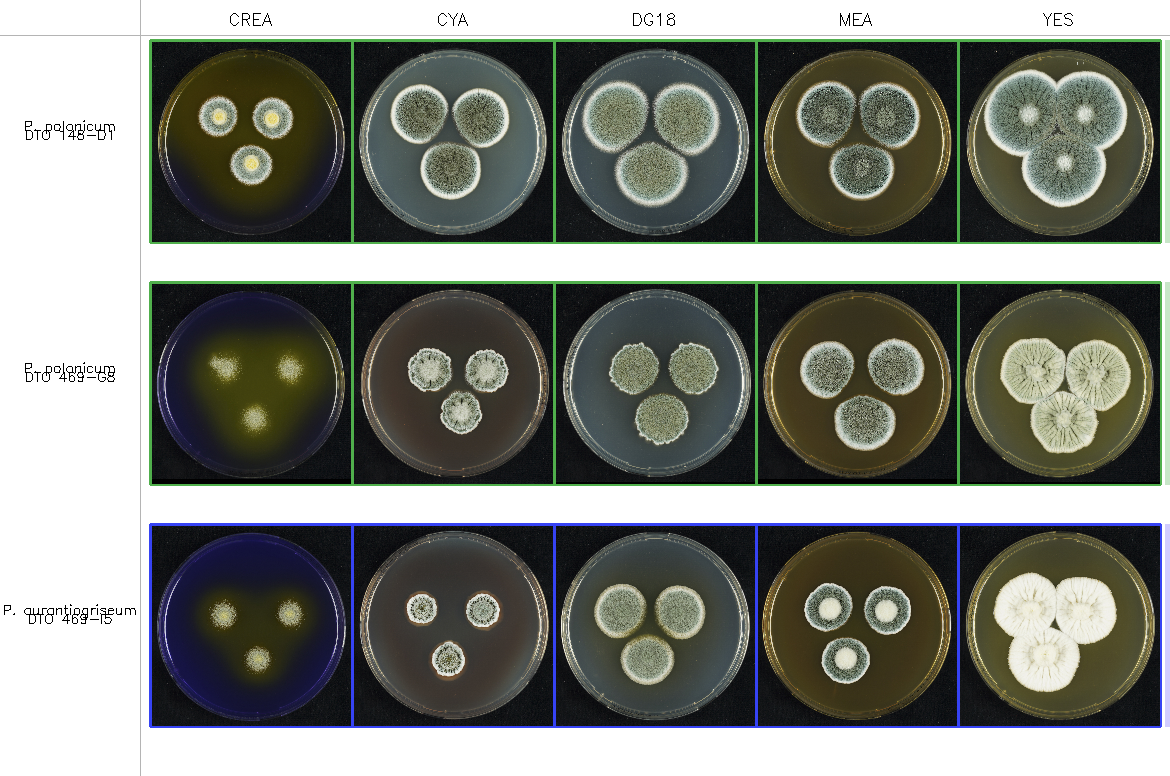
\includegraphics[width=\textwidth]{example_strain_grid.png}
      {\tiny 3 strains across 5 media. Green = same species, Red = different.}
    \end{column}
  \end{columns}
\end{frame}

% ===== SLIDE 6: EDA =====
\begin{frame}{Dataset Composition}
  \begin{columns}[T]
    \begin{column}{0.5\textwidth}
      \centering
      \textbf{Species Distribution}
      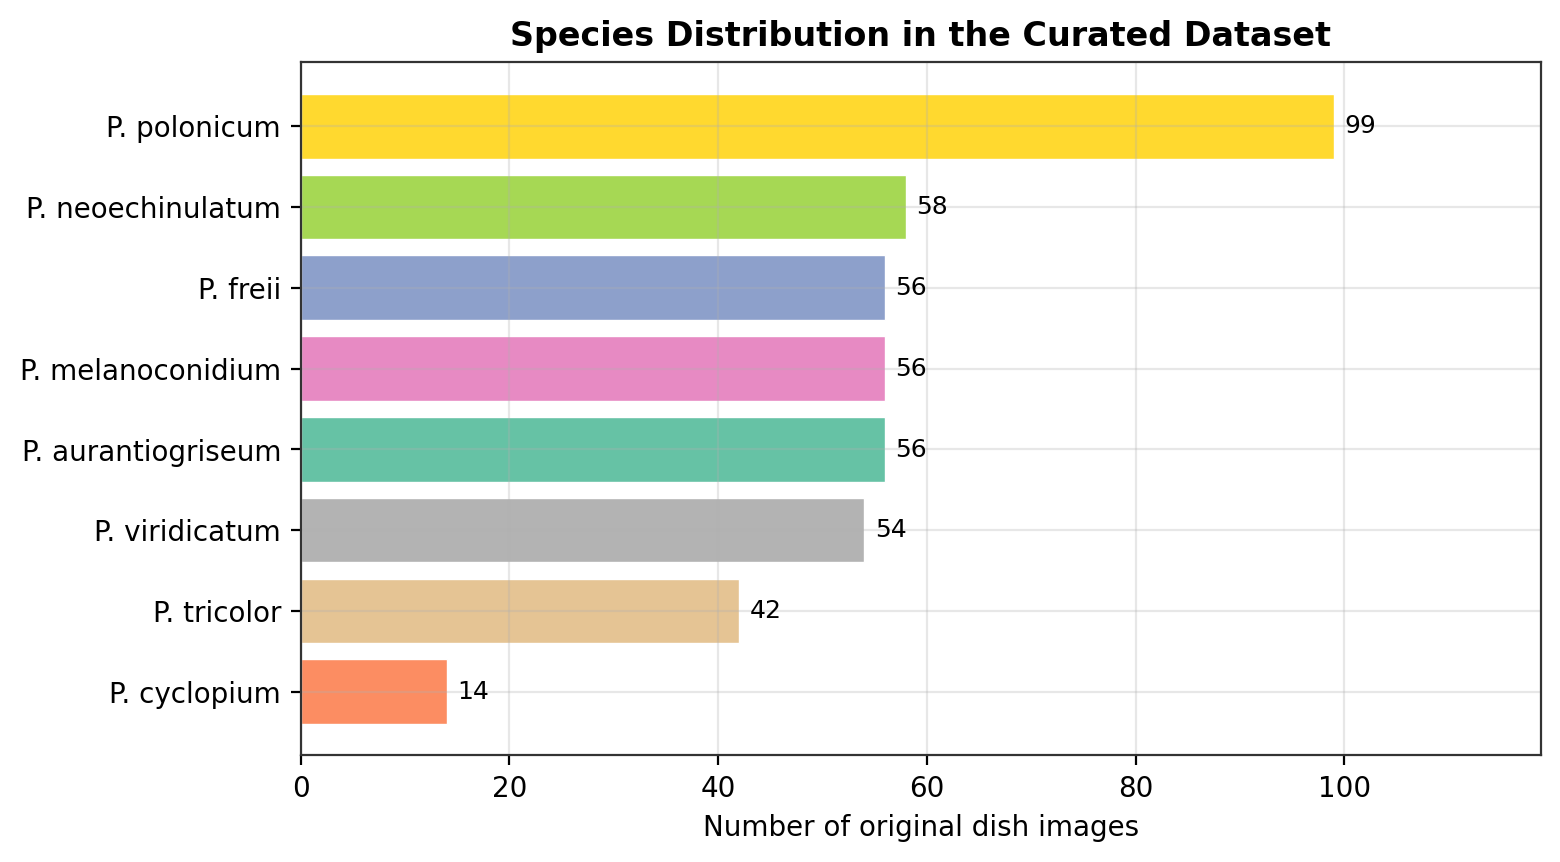
\includegraphics[width=\textwidth,height=0.55\textheight,keepaspectratio]{eda_species_distribution.png}
      {\small Class-imbalanced: 14--99 images/species}
    \end{column}
    \begin{column}{0.5\textwidth}
      \centering
      \textbf{Media Coverage}
      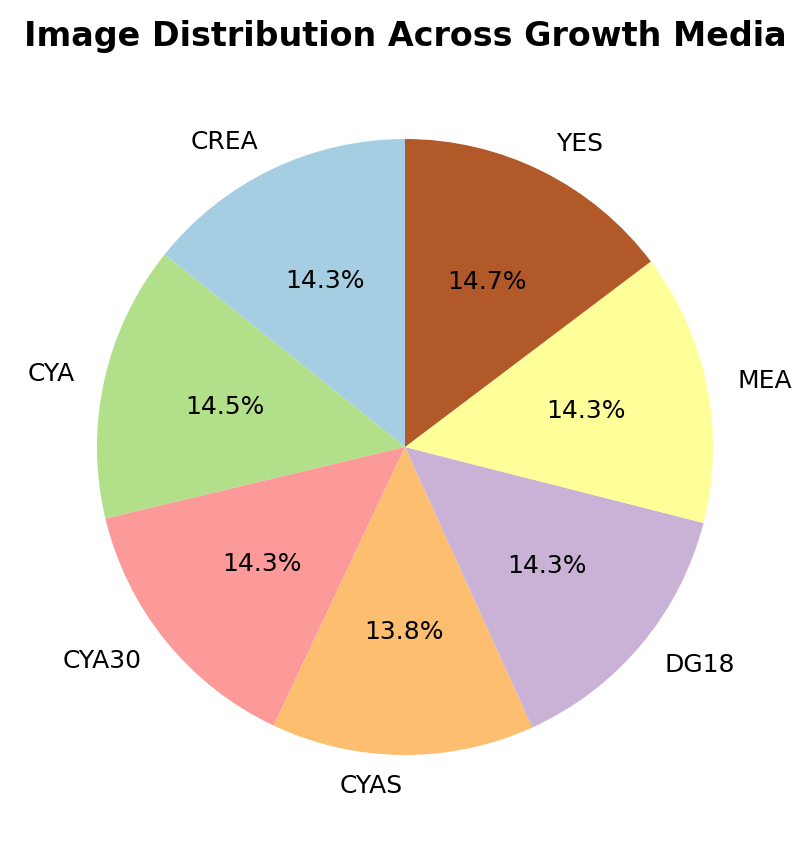
\includegraphics[width=\textwidth,height=0.55\textheight,keepaspectratio]{eda_media_distribution.png}
      {\small 7 media, 60--64 images each -- balanced}
    \end{column}
  \end{columns}
\end{frame}

% ===== SLIDE 7: FEW-SHOT =====
\begin{frame}{Few-Shot Classification Challenge}
  \begin{columns}[T]
    \begin{column}{0.48\textwidth}
      \textbf{Constraints:}
      \begin{itemize}
        \item 8 species, only 24 training strains
        \item Per-strain: 14 images (7 media $\times$ 2 angles)
        \item Mean 54 images/species, median 56
      \end{itemize}

      \textbf{Strain-level split:}
      \begin{itemize}
        \item Test: 7 held-out strains (unseen isolates)
        \item Harder than random image split
        \item Reflects real deployment
      \end{itemize}

      $\rightarrow$ Traditional CNN classifier would overfit
    \end{column}
    \begin{column}{0.52\textwidth}
      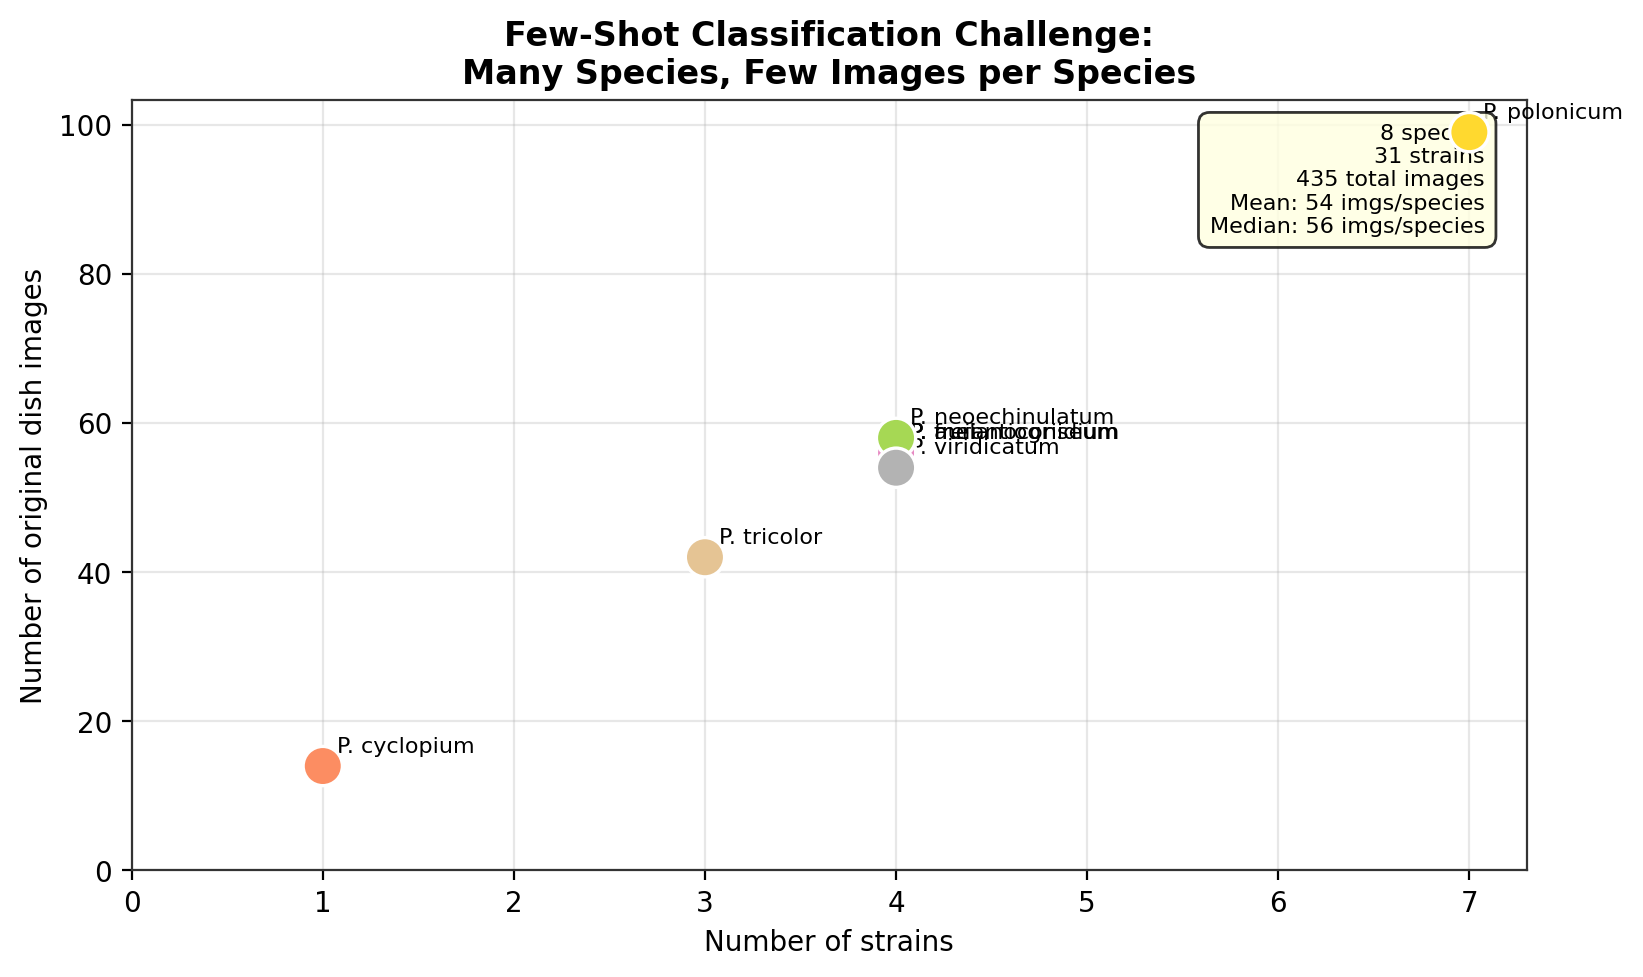
\includegraphics[width=\textwidth,height=0.35\textheight,keepaspectratio]{eda_fewshot_scatter.png}
      \vspace{0.2em}
      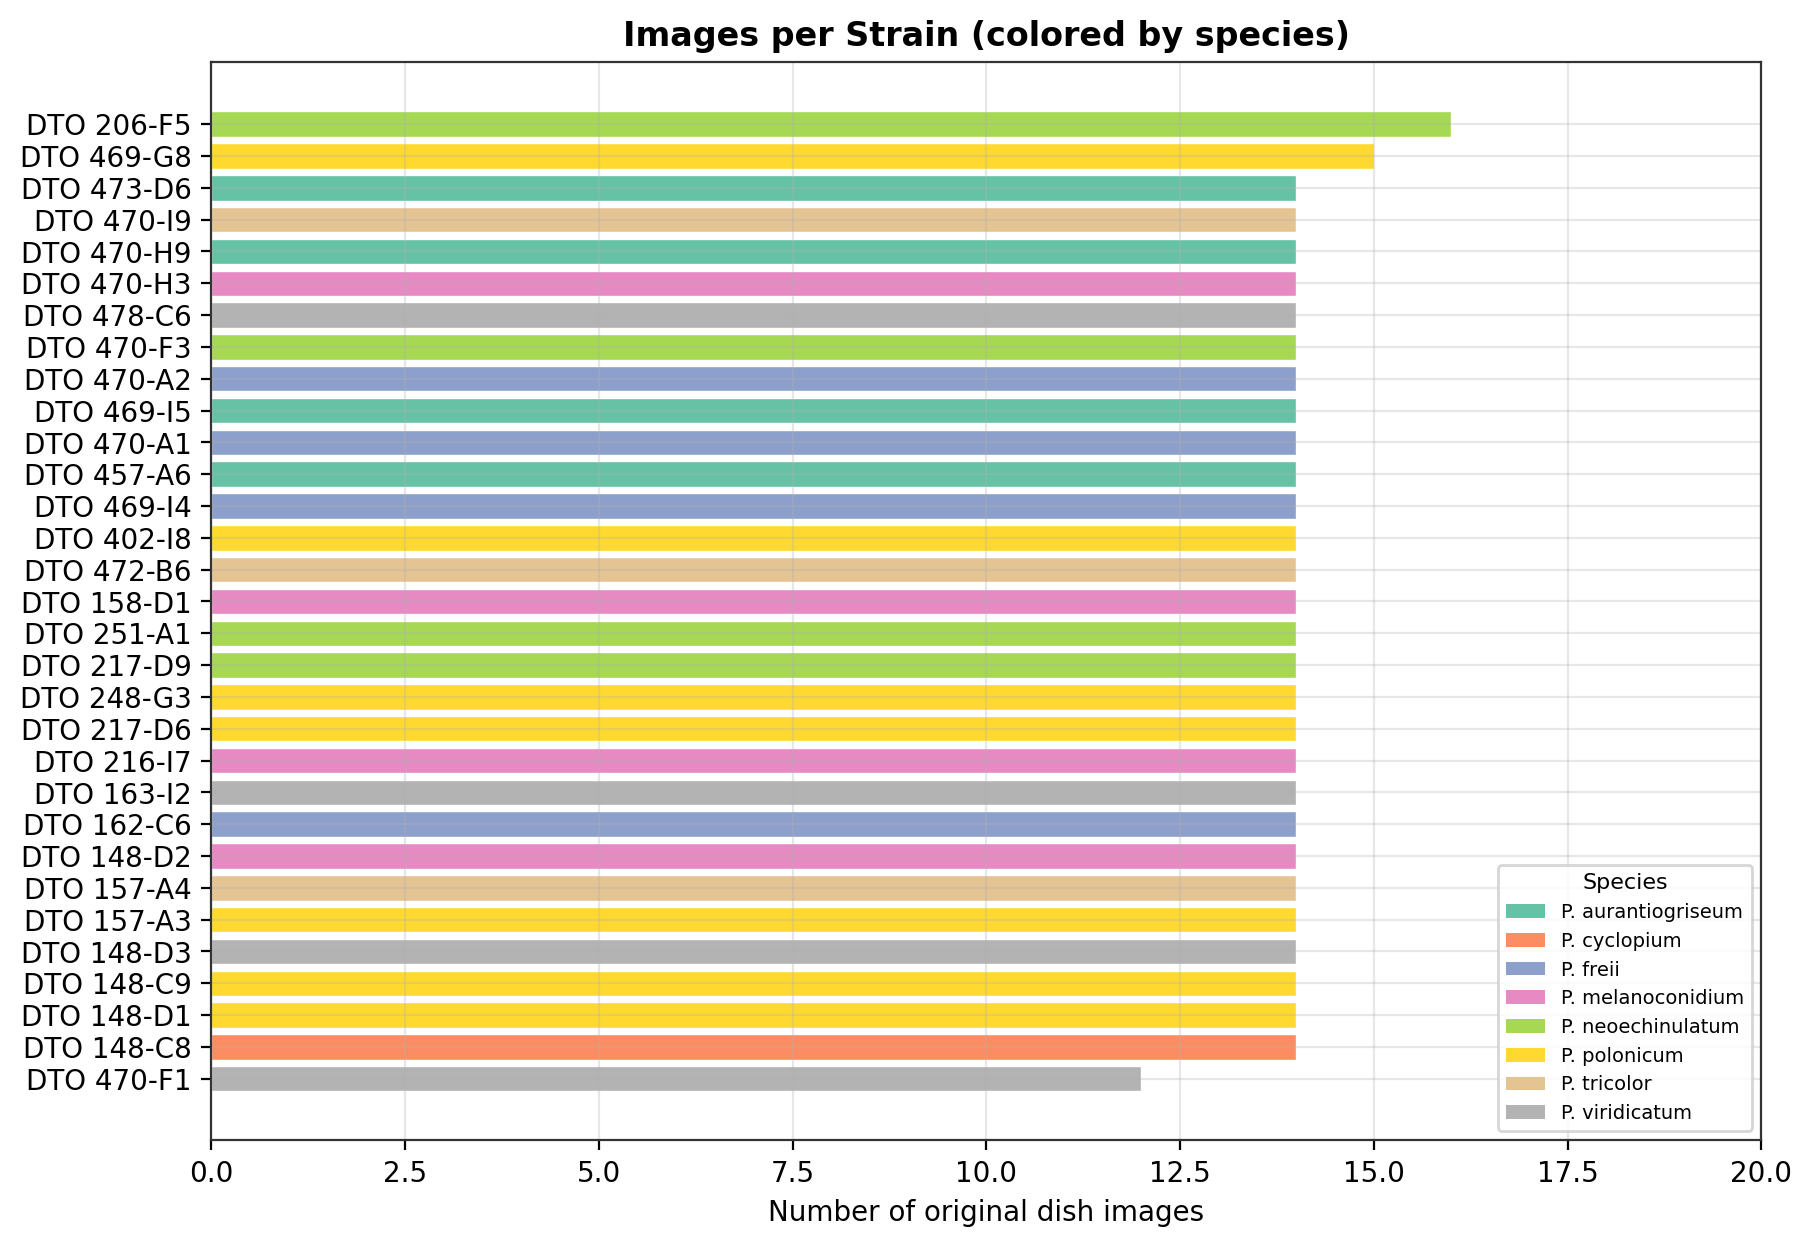
\includegraphics[width=0.85\textwidth,height=0.28\textheight,keepaspectratio]{eda_strain_distribution.png}
    \end{column}
  \end{columns}
\end{frame}

% ===== SLIDE 8: SCOPE =====
\begin{frame}{Scope -- Three Domains}
  \begin{enumerate}
    \item \textbf{Algorithmic Research}
    \begin{itemize}
      \item Colony segmentation (K-Means, contour, YOLO)
      \item Feature extraction (hand-crafted + deep learning)
      \item Vector indexing, similarity search, weighted aggregation
    \end{itemize}
    \vspace{0.3em}
    \item \textbf{System Engineering}
    \begin{itemize}
      \item Production web app: React + FastAPI + PostgreSQL + Qdrant
      \item RBAC (User / Data Owner), species catalog, feedback workflow
    \end{itemize}
    \vspace{0.3em}
    \item \textbf{Process Innovation}
    \begin{itemize}
      \item 5-agent autonomous experiment system (Autolab)
    \end{itemize}
  \end{enumerate}
\end{frame}

% ===== SLIDE 9: PIPELINE =====
\begin{frame}{Retrieval Pipeline Architecture}
  \centering
  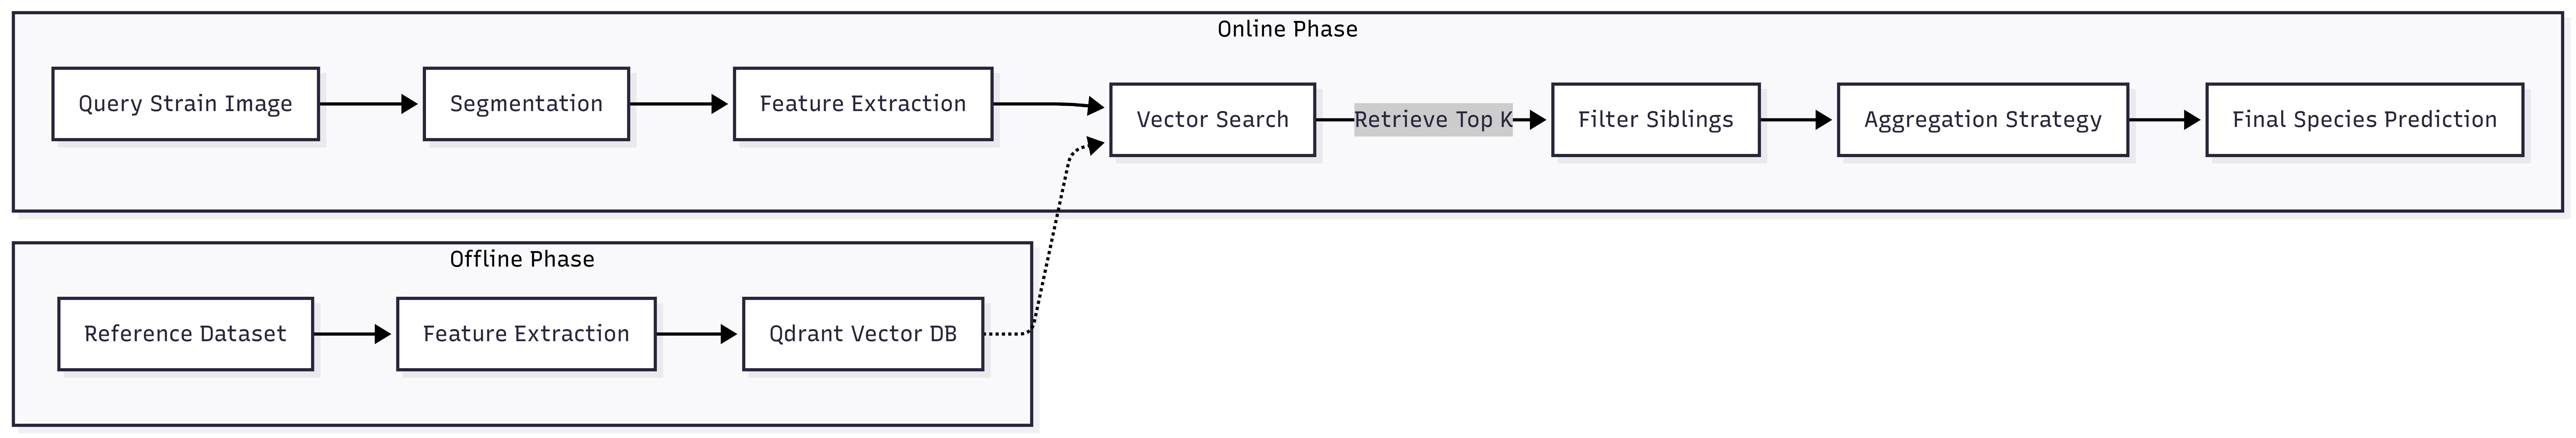
\includegraphics[width=0.8\textwidth]{query_flow.png}

  \begin{columns}[T]
    \begin{column}{0.5\textwidth}
      \textbf{Indexing Phase} (offline):
      Segment $\rightarrow$ Extract features $\rightarrow$ Store in Qdrant
    \end{column}
    \begin{column}{0.5\textwidth}
      \textbf{Query Phase} (online):
      Upload $\rightarrow$ Segment $\rightarrow$ Embed $\rightarrow$ KNN $\rightarrow$ Aggregate $\rightarrow$ Predict
    \end{column}
  \end{columns}
\end{frame}

% ===== SLIDE 10: WHY RETRIEVAL =====
\begin{frame}{Why Retrieval over Classification?}
  \begin{columns}[T]
    \begin{column}{0.48\textwidth}
      \begin{block}{Open-set}
        New species = DB insert only. No architecture change, no retraining.
      \end{block}
      \begin{block}{Interpretable}
        Shows mycologist the actual similar reference images. Expert can visually validate.
      \end{block}
      \begin{block}{Data efficient}
        No need to learn all decision boundaries. Relies on feature quality + nearest-neighbor.
      \end{block}
    \end{column}
    \begin{column}{0.52\textwidth}
      \begin{center}
        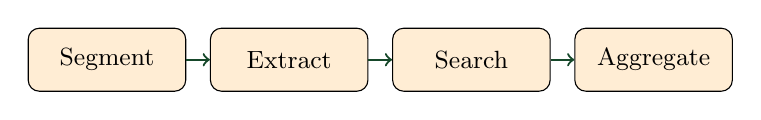
\begin{tikzpicture}[
          box/.style={draw, rounded corners, fill=mycoMid!10, minimum width=2cm, minimum height=0.8cm, align=center, font=\small},
          arrow/.style={->, thick, mycoDark}
        ]
          \node[box,fill=mycoAccent!20] (seg) {Segment};
          \node[box,right=0.3cm of seg,fill=mycoAccent!20] (feat) {Extract};
          \node[box,right=0.3cm of feat,fill=mycoAccent!20] (vec) {Search};
          \node[box,right=0.3cm of vec,fill=mycoAccent!20] (agg) {Aggregate};
          \draw[arrow] (seg) -- (feat);
          \draw[arrow] (feat) -- (vec);
          \draw[arrow] (vec) -- (agg);
        \end{tikzpicture}
      \end{center}
      \textbf{Modular design:}
      \begin{itemize}
        \item Swap extractors independently
        \item Swap segmentation freely
        \item Experiment-friendly for A/B testing
      \end{itemize}
    \end{column}
  \end{columns}
\end{frame}

% ===== SECTION: RETRIEVAL MODEL =====
\section{Retrieval Model}

% ===== SLIDE 11: PIPELINE 4 STAGES =====
\begin{frame}{Pipeline -- Four Stages}
  \begin{enumerate}
    \item \textbf{Preprocessing \& Segmentation}
    \begin{itemize}
      \item Hough Circle $\rightarrow$ background mask $\rightarrow$ K-Means colony extraction
      \item Local K=2 Shrink for halo removal (MEA, YES)
      \item Alternatives: Contour (Canny), YOLOv8n-seg
    \end{itemize}
    \vspace{0.3em}
    \item \textbf{Feature Extraction}
    \begin{itemize}
      \item Hand-crafted: HOG (3,780d), Gabor (40d), ColorHistHS (64d)
      \item Deep: ResNet50, MobileNetV2, EfficientNetB1 -- fine-tuned
    \end{itemize}
    \vspace{0.3em}
    \item \textbf{Vector Database (Qdrant)}
    \begin{itemize}
      \item Cosine similarity, 13 named vectors per point, sibling filtering
    \end{itemize}
    \vspace{0.3em}
    \item \textbf{Aggregation}
    \begin{itemize}
      \item Weighted sum of per-segment neighbor similarities, normalized by frequency
    \end{itemize}
  \end{enumerate}
\end{frame}

% ===== SLIDE 12: SEGMENTATION =====
\begin{frame}{Colony Segmentation}
  \begin{table}
    \centering
    \begin{tabular}{@{}lccc@{}}
      \toprule
      \textbf{Method} & \textbf{Colonies} & \textbf{Flare-robust?} & \textbf{Labels?} \\
      \midrule
      K-Means (K=2, HSV) & 3 & Partial (Local K=2) & No \\
      Contour (Canny + Circ.) & 2--3 & Yes (edge-based) & No \\
      YOLOv8n-seg & Variable & Yes (learned) & Yes \\
      \bottomrule
    \end{tabular}
  \end{table}

  \textbf{Local K=2 Shrink} (key innovation):
  \begin{itemize}
    \item Bright colonies on MEA/YES create light halos
    \item Second K=2 on value channel within each candidate region
    \item Morphological erosion strips borderline halo pixels
  \end{itemize}

  {\small \textbf{Production choice:} K-Means + Local K=2. YOLO reserved for cross-validation.}
\end{frame}

% ===== SLIDE 13: FEATURE EXTRACTORS =====
\begin{frame}{Feature Extractors Comparison}
  \begin{table}
    \centering
    \small
    \begin{tabular}{@{}lcrr@{}}
      \toprule
      \textbf{Extractor} & \textbf{Dim} & \textbf{Accuracy} & \textbf{$\Delta$ Pretrained} \\
      \midrule
      \rowcolor{mycoLight!30}
      \textbf{EfficientNetB1 (FT)} & 1,280 & \textbf{83.3\%} & \textbf{+20.3\%} \\
      ResNet50 (FT) & 2,048 & 78.6\% & +15.6\% \\
      MobileNetV2 (FT) & 1,280 & 78.6\% & +18.6\% \\
      HS+ResNet50 (Hybrid) & 2,112 & 72\% & -- \\
      ColorHistHS & 64 & 65\% & -- \\
      ResNet50 (Pretrained) & 2,048 & 63\% & baseline \\
      Triplet Loss (EffNetB1) & 128 & 64.3\% & -- \\
      Gabor & 40 & 55\% & -- \\
      HOG & 3,780 & 52\% & -- \\
      \bottomrule
    \end{tabular}
  \end{table}
  \vspace{0.2em}
  \textbf{Key:} Fine-tuning = +15--20\%. Triplet loss fails (19\% worse) on small datasets.
\end{frame}

% ===== SLIDE 14: FINE-TUNING =====
\begin{frame}{Fine-Tuning \& Training}
  \begin{columns}[T]
    \begin{column}{0.52\textwidth}
      \textbf{Setup:}
      \begin{itemize}
        \item 1,011 training images (24 strains)
        \item 294 validation images (7 held-out strains)
        \item Augmentation: HFlip(0.5), Rot$\pm$10$^\circ$
        \item CrossEntropyLoss, Adam, lr=0.0001
        \item 50 epochs max, early stopping patience=10
      \end{itemize}

      \textbf{Why not triplet loss?}
      \begin{itemize}
        \item Needs 10$\times$ more data than classification
        \item Reduced dim (128 vs 1280) limits capacity
        \item No hard negative mining
        \item Class imbalance biases triplet sampling
      \end{itemize}
    \end{column}
    \begin{column}{0.48\textwidth}
      \begin{table}
        \centering
        \small
        \begin{tabular}{@{}lcc@{}}
          \toprule
          \textbf{Model} & \textbf{Acc.} & \textbf{Params} \\
          \midrule
          EfficientNetB1 & 83.3\% & 7.8M \\
          ResNet50 & 78.6\% & 25.6M \\
          MobileNetV2 & 78.6\% & 3.5M \\
          \bottomrule
        \end{tabular}
      \end{table}
      \begin{block}{MobileNetV2}
        78.6\% at 7$\times$ fewer params. Edge-deployable.
      \end{block}
    \end{column}
  \end{columns}
\end{frame}

% ===== SLIDE 15: VECTOR DB =====
\begin{frame}{Vector Database \& Aggregation}
  \begin{columns}[T]
    \begin{column}{0.5\textwidth}
      \textbf{Qdrant:}
      \begin{itemize}
        \item 1,305 colony segments indexed
        \item 13 named vectors per point
        \item Dynamic filtering (sibling exclusion)
        \item Environment filter: same-media / all-media
      \end{itemize}

      \textbf{Environment Strategies:}
      \begin{itemize}
        \item E1 (All): train on all media $\rightarrow$ \textbf{best}
        \item E2 (Balanced): equal per-media samples
        \item E3 (Single-Env): test one medium
        \item E4 (Leave-One-Out): exclude one medium
      \end{itemize}
    \end{column}
    \begin{column}{0.5\textwidth}
      \textbf{Weighted Aggregation:}
      \[
      S_c = \frac{\sum s_{i,j} \cdot \mathbb{1}[c_{i,j}=c]}{\sum \mathbb{1}[c_{i,j}=c]}
      \]
      \begin{itemize}
        \item Normalizes by frequency
        \item Typical: 18 segments per strain
        \item Per-segment KNN $\rightarrow$ merged species score
      \end{itemize}

      \textbf{Optimal $k$: 7} (cross-validated)
    \end{column}
  \end{columns}
\end{frame}

% ===== SLIDE 16: STAIRCASE =====
\begin{frame}{Autoresearch -- Staircase Chart}
  \centering
  \textbf{Hundreds of combinations tested:} distance metrics, aggregation, $k$-values, media filters

  \vspace{0.5em}
  \begin{itemize}
    \item Each dot = one experiment (formula $\times$ algorithm pair)
    \item Green dots = new best F1 $\rightarrow$ staircase steps up
    \item Gray dots = below running best
    \item Labels = strategy name on each green dot
  \end{itemize}
  \vspace{0.5em}

  {\small Staircase chart from \texttt{results/autoresearch/retrieval.csv}}
\end{frame}

% ===== SLIDE 17: PERFORMANCE =====
\begin{frame}{Overall Performance -- EfficientNetB1}
  \begin{columns}[T]
    \begin{column}{0.45\textwidth}
      \begin{table}
        \centering
        \small
        \begin{tabular}{@{}lc@{}}
          \toprule
          \textbf{Species} & \textbf{Acc.} \\
          \midrule
          \textit{P. polonicum} & 100\% \\
          \textit{P. freii} & 100\% \\
          \textit{P. neoechinulatum} & 100\% \\
          \textit{P. aurantiogriseum} & 83\% \\
          \textit{P. viridicatum} & 83\% \\
          \textit{P. tricolor} & 67\% \\
          \textit{P. melanoconidium} & 50\% \\
          \midrule
          \rowcolor{mycoLight!20}
          \textbf{Overall} & \textbf{83.3\%} \\
          \bottomrule
        \end{tabular}
      \end{table}
    \end{column}
    \begin{column}{0.55\textwidth}
      \textbf{Key findings:}
      \begin{itemize}
        \item \textbf{Fine-tuning critical:} +15--20\%
        \item \textbf{MobileNetV2:} 78.6\% at 3.5M params
        \item \textbf{Hand-crafted plateau:} max 65\%
        \item \textbf{Triplet loss:} 19\% worse
      \end{itemize}

      \textbf{Confusions:}
      \begin{itemize}
        \item \textit{P. melanoconidium} $\leftrightarrow$ \textit{P. aurantiogriseum} (dark colonies)
        \item \textit{P. tricolor} $\leftrightarrow$ \textit{P. viridicatum} (green pigment)
      \end{itemize}
    \end{column}
  \end{columns}
\end{frame}

% ===== SLIDE 18: CROSS-VAL =====
\begin{frame}{5-Fold Cross-Validation}
  \begin{table}
    \centering
    \small
    \begin{tabular}{@{}lccrrr@{}}
      \toprule
      \textbf{Env} & \textbf{Agg} & \textbf{K} & \textbf{Mean} & \textbf{Std} & \textbf{Max} \\
      \midrule
      \rowcolor{mycoLight!20}
      E1 & weighted & 7 & 0.833 & 0.052 & 0.905 \\
      E1 & weighted & 9 & 0.829 & 0.048 & 0.905 \\
      E1 & uni & 5 & 0.810 & 0.065 & 0.905 \\
      E2 & weighted & 9 & 0.805 & 0.072 & 0.905 \\
      \bottomrule
    \end{tabular}
  \end{table}

  \textbf{Conclusions:}
  \begin{itemize}
    \item \textbf{E1 (all environments)} beats E2 -- diversity helps
    \item \textbf{Weighted aggregation} outperforms uniform
    \item \textbf{$k=7$} optimal: smaller noisy, larger dissimilar neighbors
    \item \textbf{Stable:} std 5--7\% across folds
  \end{itemize}
  {\small 100 total runs: 5 folds $\times$ 2 env $\times$ 2 agg $\times$ 5 K values}
\end{frame}

% ===== SLIDE 19: t-SNE =====
\begin{frame}{Feature Space \& Confusion Analysis}
  \begin{columns}[T]
    \begin{column}{0.5\textwidth}
      \textbf{t-SNE (ResNet50 fine-tuned):}
      \begin{itemize}
        \item Clear clusters: \textit{P. polonicum, freii, neoechinulatum}
        \item Overlap: \textit{P. melanoconidium} / \textit{P. aurantiogriseum}
        \item \textbf{No environment clustering!}
      \end{itemize}

      $\rightarrow$ Model learns \textbf{environment-invariant, species-discriminative} features
    \end{column}
    \begin{column}{0.5\textwidth}
      \textbf{Bottleneck species:}
      \begin{itemize}
        \item 3 species at \textbf{100\%} (perfect)
        \item 2 at \textbf{83\%}
        \item \textit{P. tricolor}: 67\%
        \item \textit{P. melanoconidium}: 50\% -- hardest
      \end{itemize}

      Dark-colony species visually indistinguishable even for experts. Hard negative mining or two-stage classifier could help.
    \end{column}
  \end{columns}
\end{frame}

% ===== SECTION: WEB APPLICATION =====
\section{Web Application}

% ===== SLIDE 20: ARCHITECTURE =====
\begin{frame}{System Architecture}
  \centering
  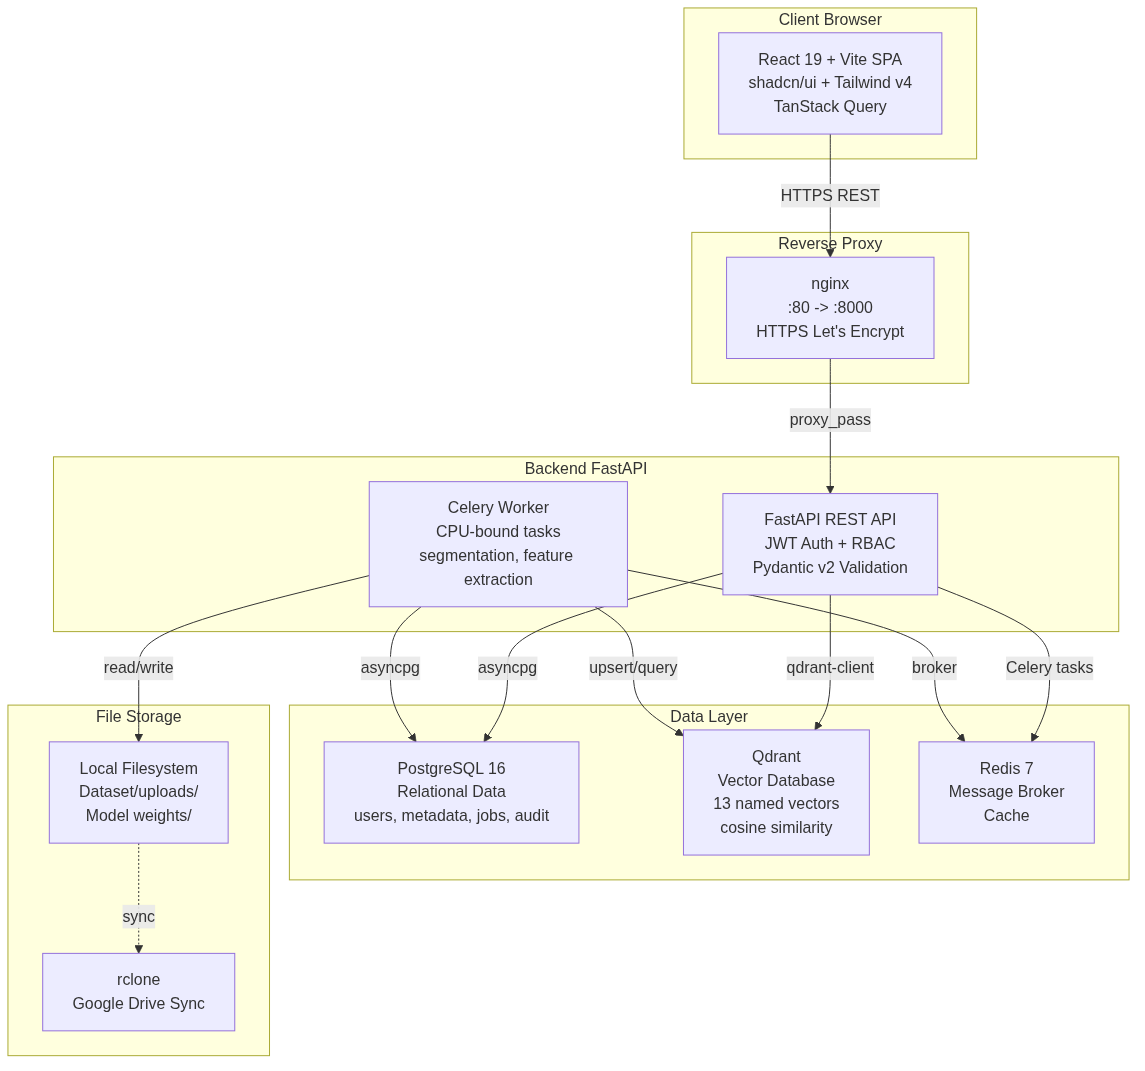
\includegraphics[width=0.65\textwidth,height=0.4\textheight,keepaspectratio]{ch03_architecture.png}

  \begin{columns}[T]
    \begin{column}{0.5\textwidth}
      \textbf{6 services:}
      \begin{itemize}
        \item React 19 SPA (Vite + TypeScript)
        \item FastAPI (Python 3.13)
        \item PostgreSQL (governance)
        \item Qdrant (vector search)
        \item Redis + Celery (async)
      \end{itemize}
    \end{column}
    \begin{column}{0.5\textwidth}
      \textbf{Dual-DB strategy:}
      \begin{itemize}
        \item PostgreSQL: ACID, RBAC, audit
        \item Qdrant: 1,280-dim embeddings
        \item Bridge table prevents drift
      \end{itemize}
    \end{column}
  \end{columns}
\end{frame}

% ===== SLIDE 21: TECH STACK =====
\begin{frame}{Technology Stack}
  \begin{table}
    \centering
    \small
    \begin{tabular}{@{}lll@{}}
      \toprule
      \textbf{Layer} & \textbf{Tech} & \textbf{Why} \\
      \midrule
      Frontend & React 19 + Vite + TS & SPA, HMR, type safety \\
      UI & shadcn/ui + Tailwind v4 & Accessible, utility-first \\
      Data & TanStack Query & Caching, auto-refetch \\
      Backend & FastAPI (async) & Auto-docs, Pydantic v2 \\
      ORM & SQLAlchemy 2.0 async & DeclarativeBase \\
      Vector DB & Qdrant & Cosine KNN, named vectors \\
      Tasks & Celery + Redis & Retries, monitoring \\
      Auth & python-jose + bcrypt & JWT access/refresh \\
      CV & OpenCV + scikit-learn & KMeans, contour \\
      Deploy & Docker Compose & Single-VM reproducible \\
      CI/CD & GitHub Actions & Lint, typecheck, test \\
      \bottomrule
    \end{tabular}
  \end{table}
\end{frame}

% ===== SLIDE 22: DATABASE =====
\begin{frame}{Database Design}
  \begin{columns}[T]
    \begin{column}{0.4\textwidth}
      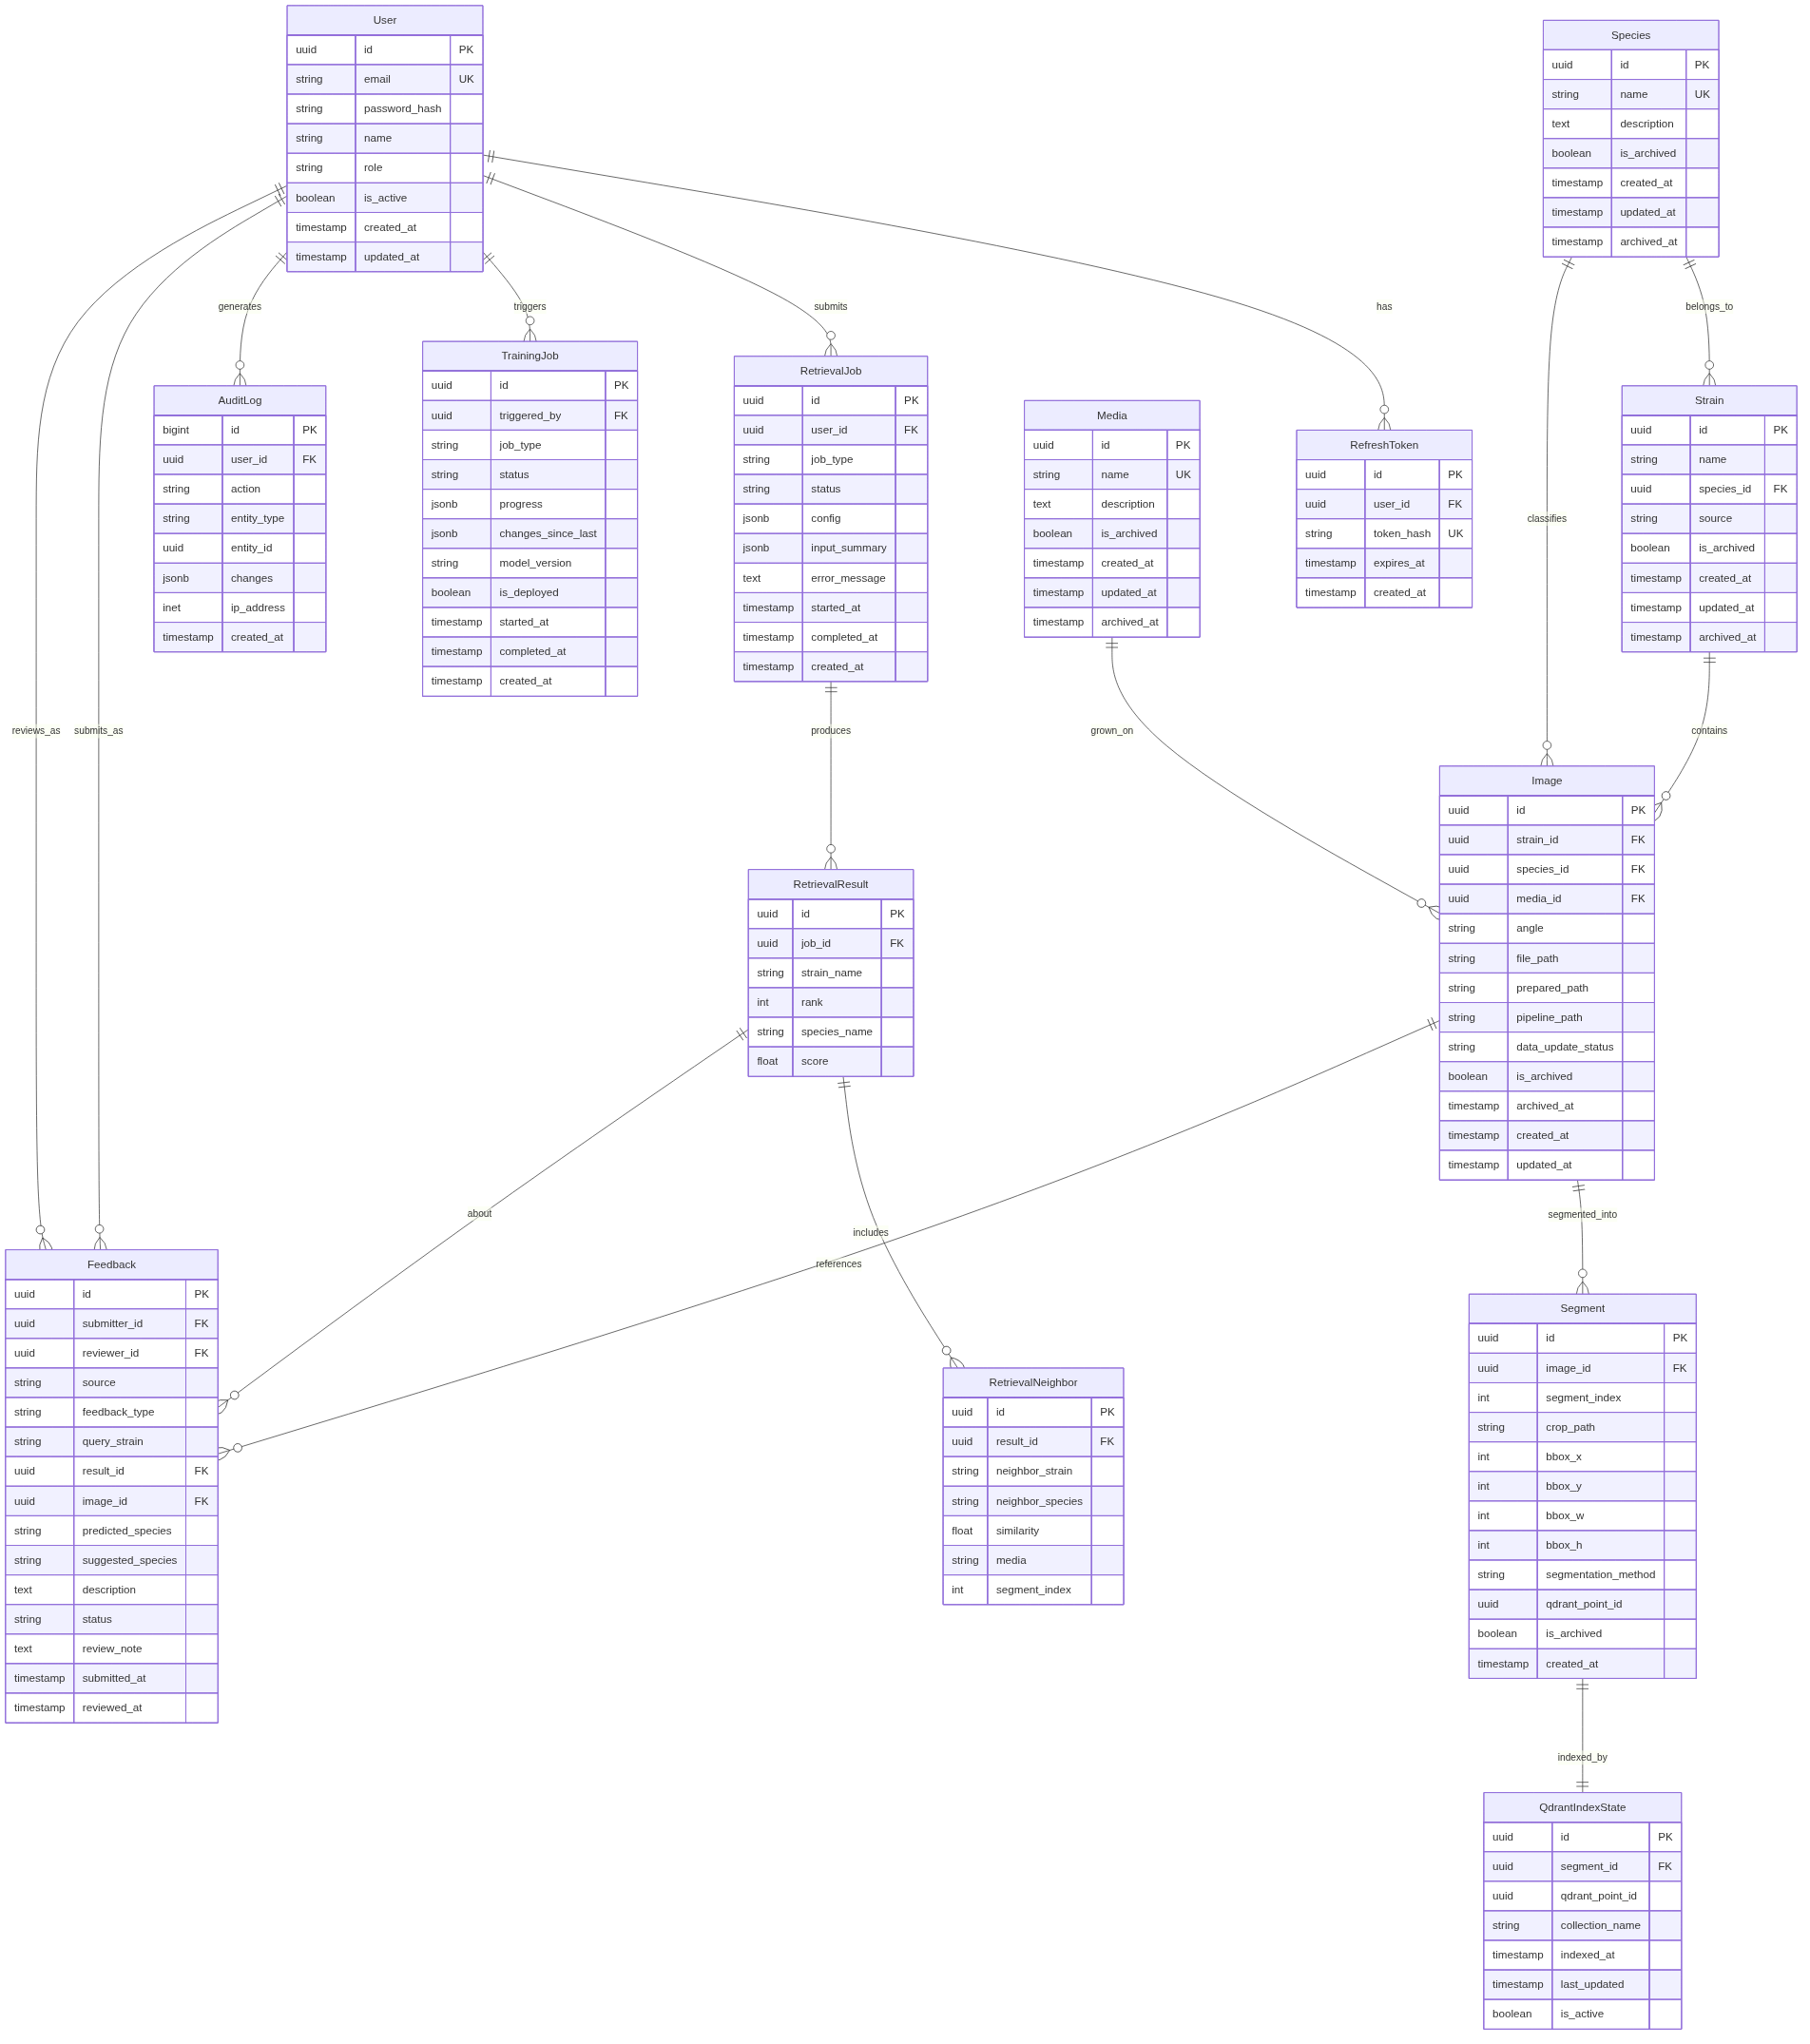
\includegraphics[width=\textwidth,height=0.72\textheight,keepaspectratio]{ch03_erd.png}
    \end{column}
    \begin{column}{0.6\textwidth}
      \textbf{14 tables:}
      \begin{itemize}
        \item Core: Users, Species, Media, Strains, Images, Segments
        \item Jobs: RetrievalJob, RetrievalResult, RetrievalNeighbor
        \item Governance: Feedback, AuditLog, TrainingJob
        \item State: QdrantIndexState, SystemState
      \end{itemize}

      \textbf{Key patterns:}
      \begin{itemize}
        \item UUIDv4 PKs -- distributed-safe
        \item Soft delete (\texttt{is\_archived}) -- no permanent deletion
        \item JSONB for config, progress, diffs
        \item \texttt{data\_update\_status} drives Qdrant re-index
      \end{itemize}
    \end{column}
  \end{columns}
\end{frame}

% ===== SLIDE 23: API + AUTH =====
\begin{frame}{API Design \& Authentication}
  \begin{columns}[T]
    \begin{column}{0.45\textwidth}
      \textbf{REST API -- \texttt{/api/v1/}:}
      \begin{itemize}
        \item 47 endpoints, 9 resource groups
        \item RFC 7807 error format
        \item Async job: 202 Accepted + polling
      \end{itemize}
      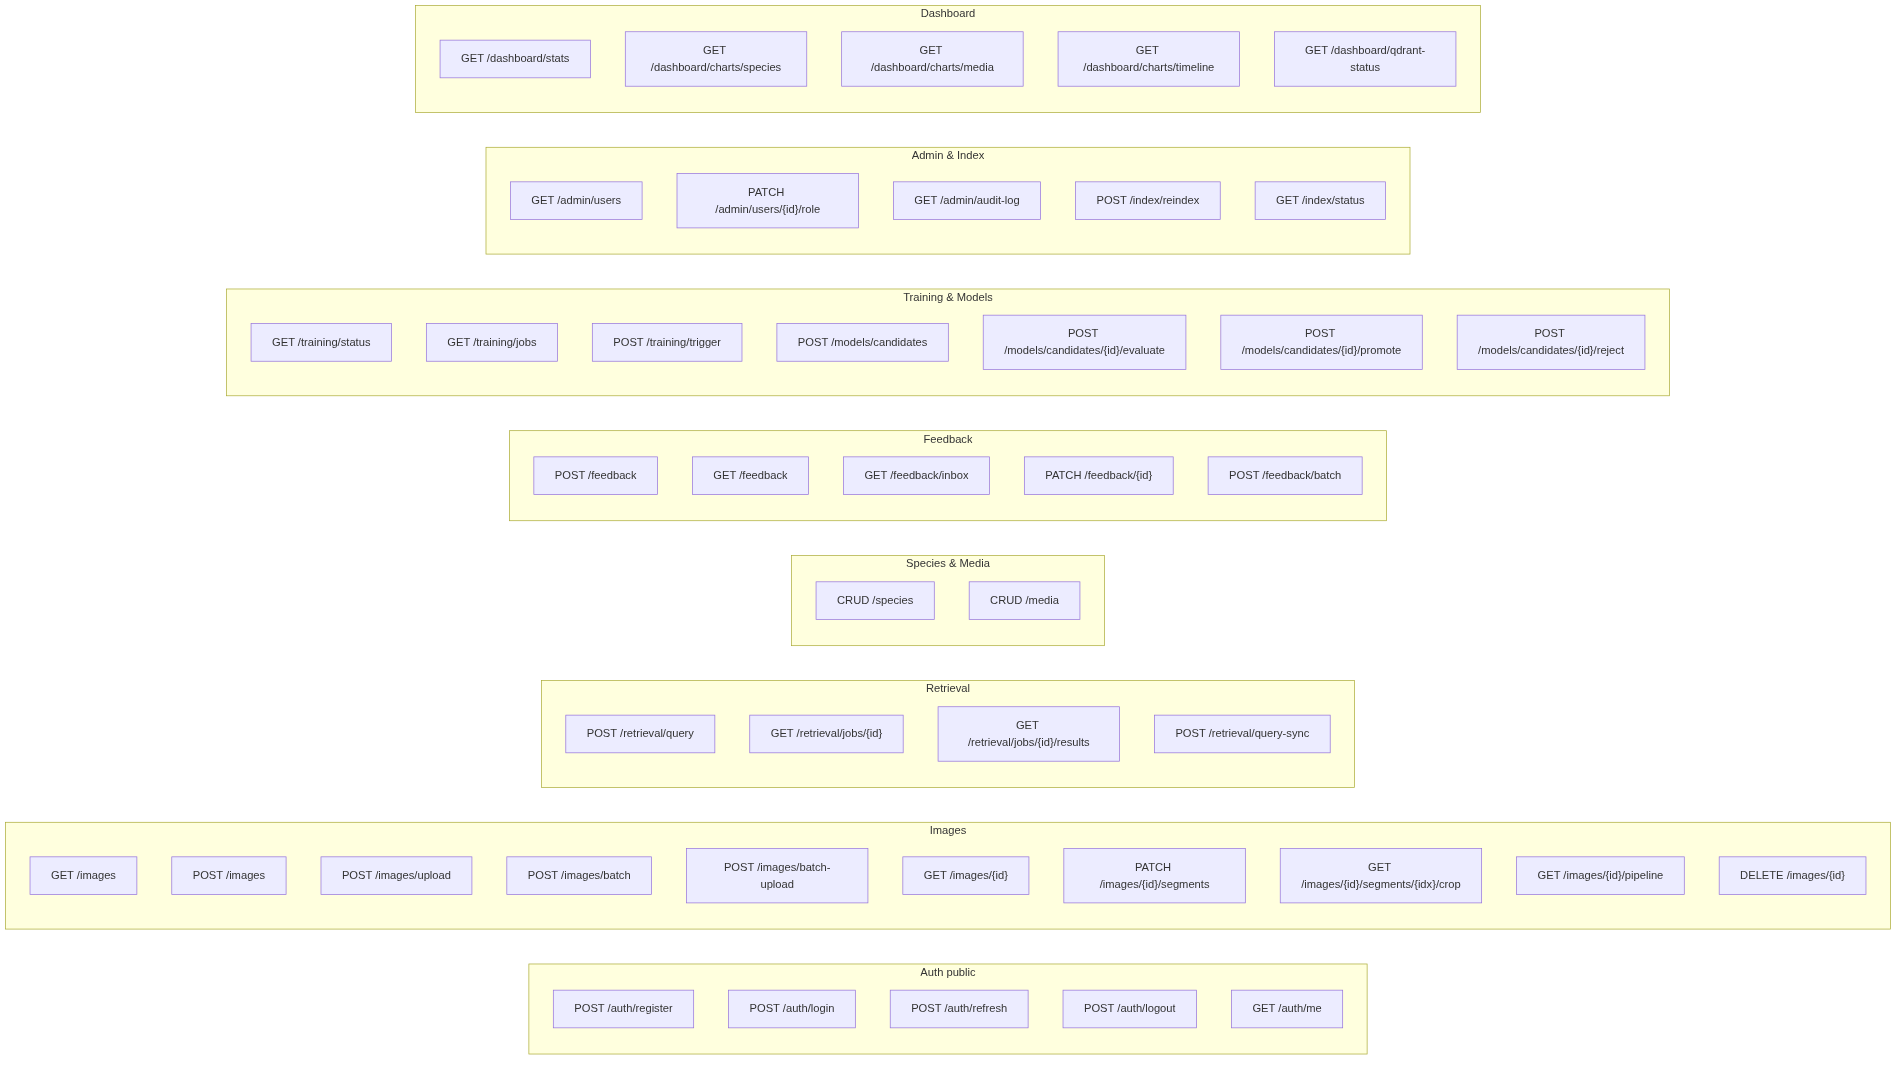
\includegraphics[width=\textwidth,height=0.38\textheight,keepaspectratio]{ch03_api_map.png}
    \end{column}
    \begin{column}{0.55\textwidth}
      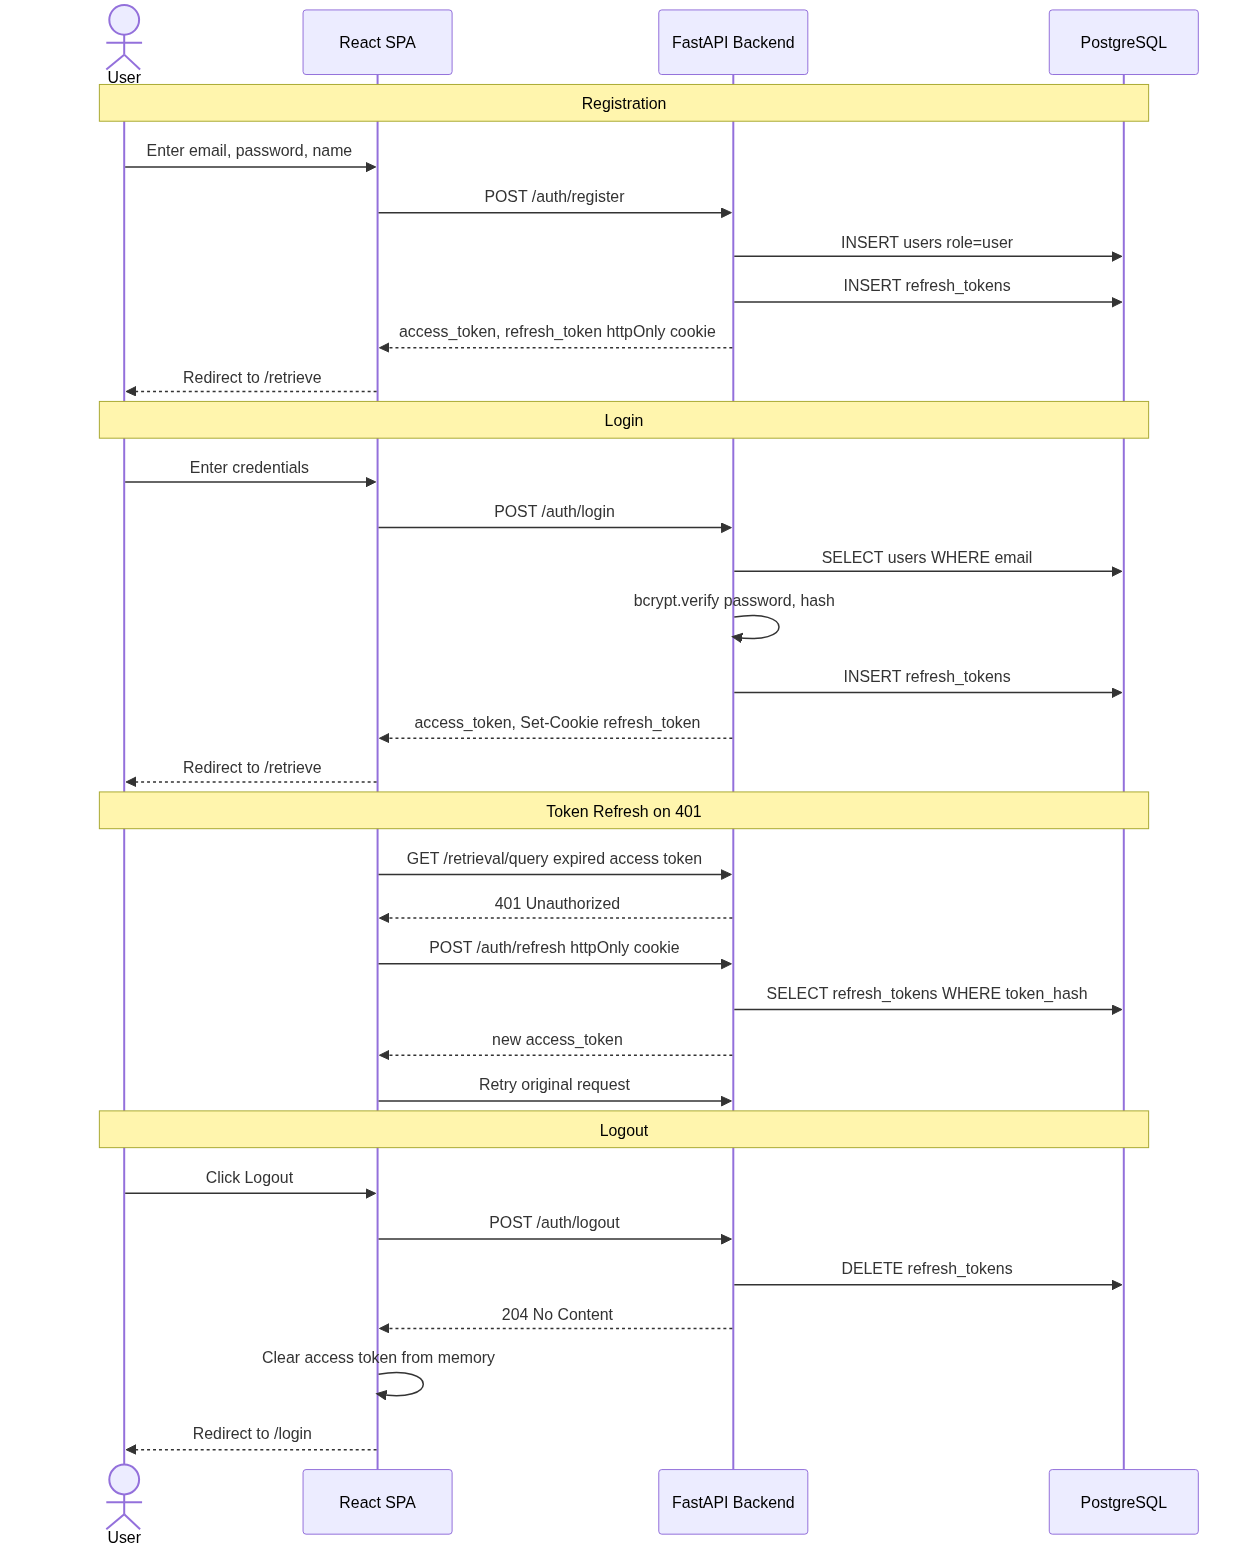
\includegraphics[width=\textwidth,height=0.38\textheight,keepaspectratio]{ch03_auth_sequence.png}
      \begin{itemize}
        \item Access token: 1h, HS256
        \item Refresh token: 30d, httpOnly cookie
        \item RBAC: User / Data Owner roles
      \end{itemize}
    \end{column}
  \end{columns}
\end{frame}

% ===== SLIDE 24: FRONTEND =====
\begin{frame}{Frontend Application}
  \begin{columns}[T]
    \begin{column}{0.45\textwidth}
      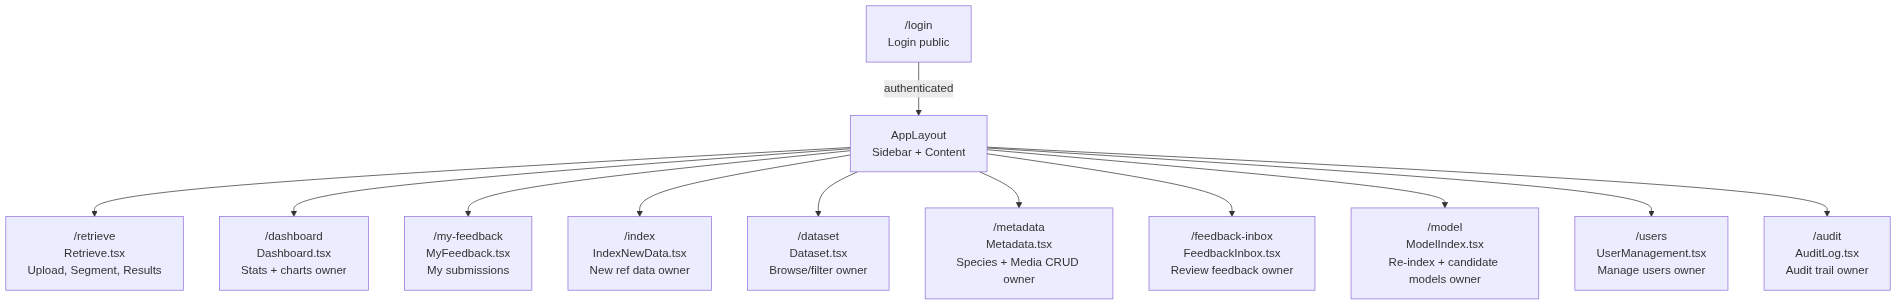
\includegraphics[width=\textwidth,height=0.35\textheight,keepaspectratio]{ch03_frontend_routes.png}
    \end{column}
    \begin{column}{0.55\textwidth}
      \textbf{11 pages, role-gated:}
      \begin{itemize}
        \item \textbf{Retrieve} -- 3-step upload/review/results
        \item \textbf{Dataset} -- filter, group, archive
        \item \textbf{Dashboard} -- SVG charts, index status
        \item \textbf{Model Index} -- re-index, candidate models
        \item \textbf{Feedback} -- review user contributions
        \item \textbf{Metadata / Users / Audit} -- owner-only
      \end{itemize}
      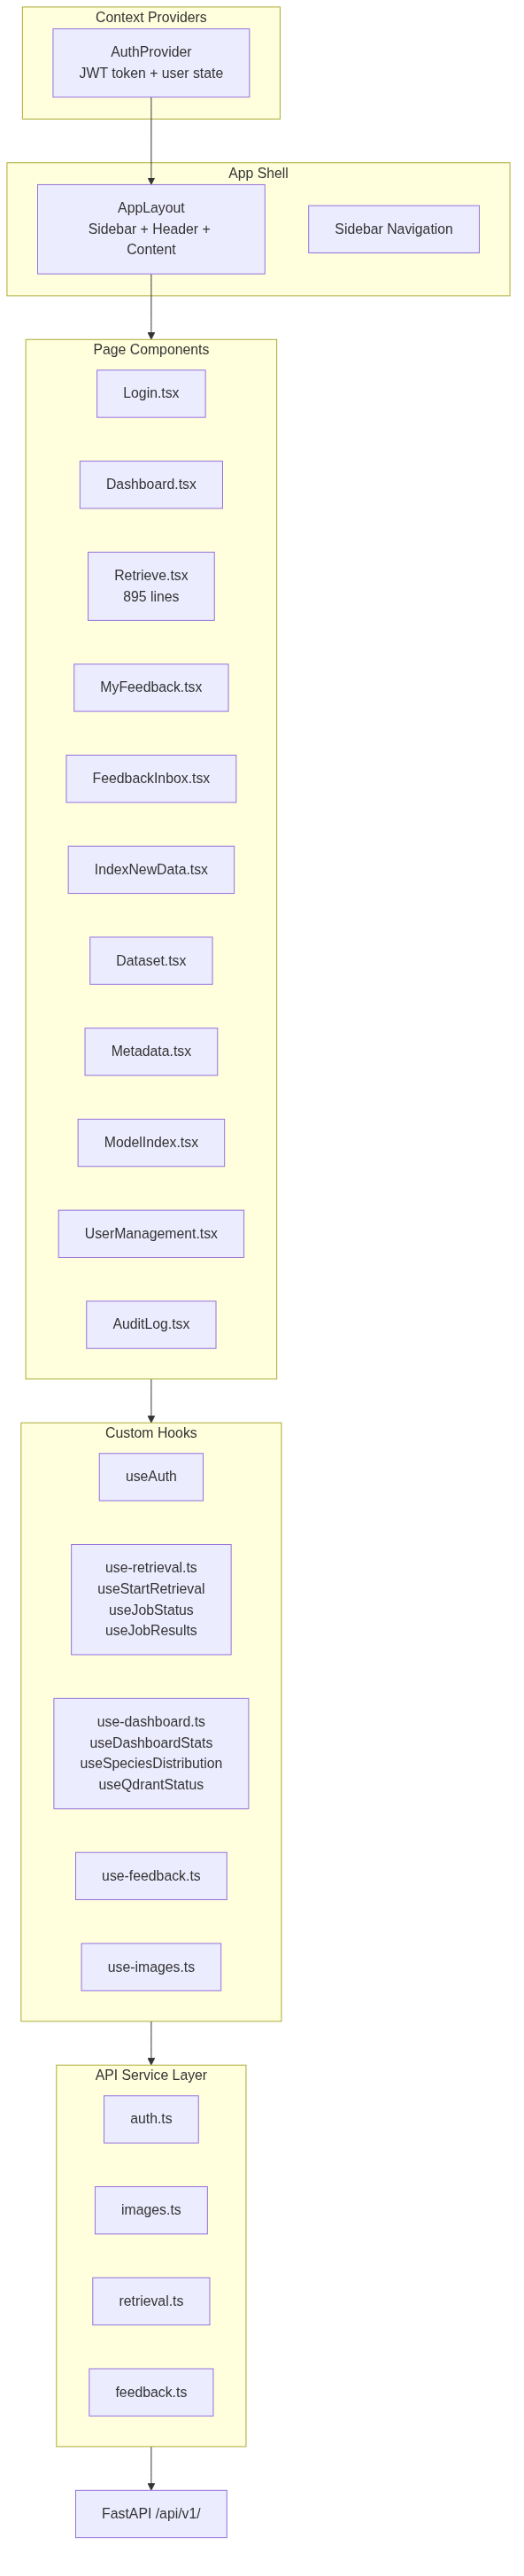
\includegraphics[width=\textwidth,height=0.28\textheight,keepaspectratio]{ch03_component_architecture.png}
    \end{column}
  \end{columns}
\end{frame}

% ===== SLIDE 25: DEPLOYMENT =====
\begin{frame}{Deployment \& CI/CD}
  \begin{columns}[T]
    \begin{column}{0.52\textwidth}
      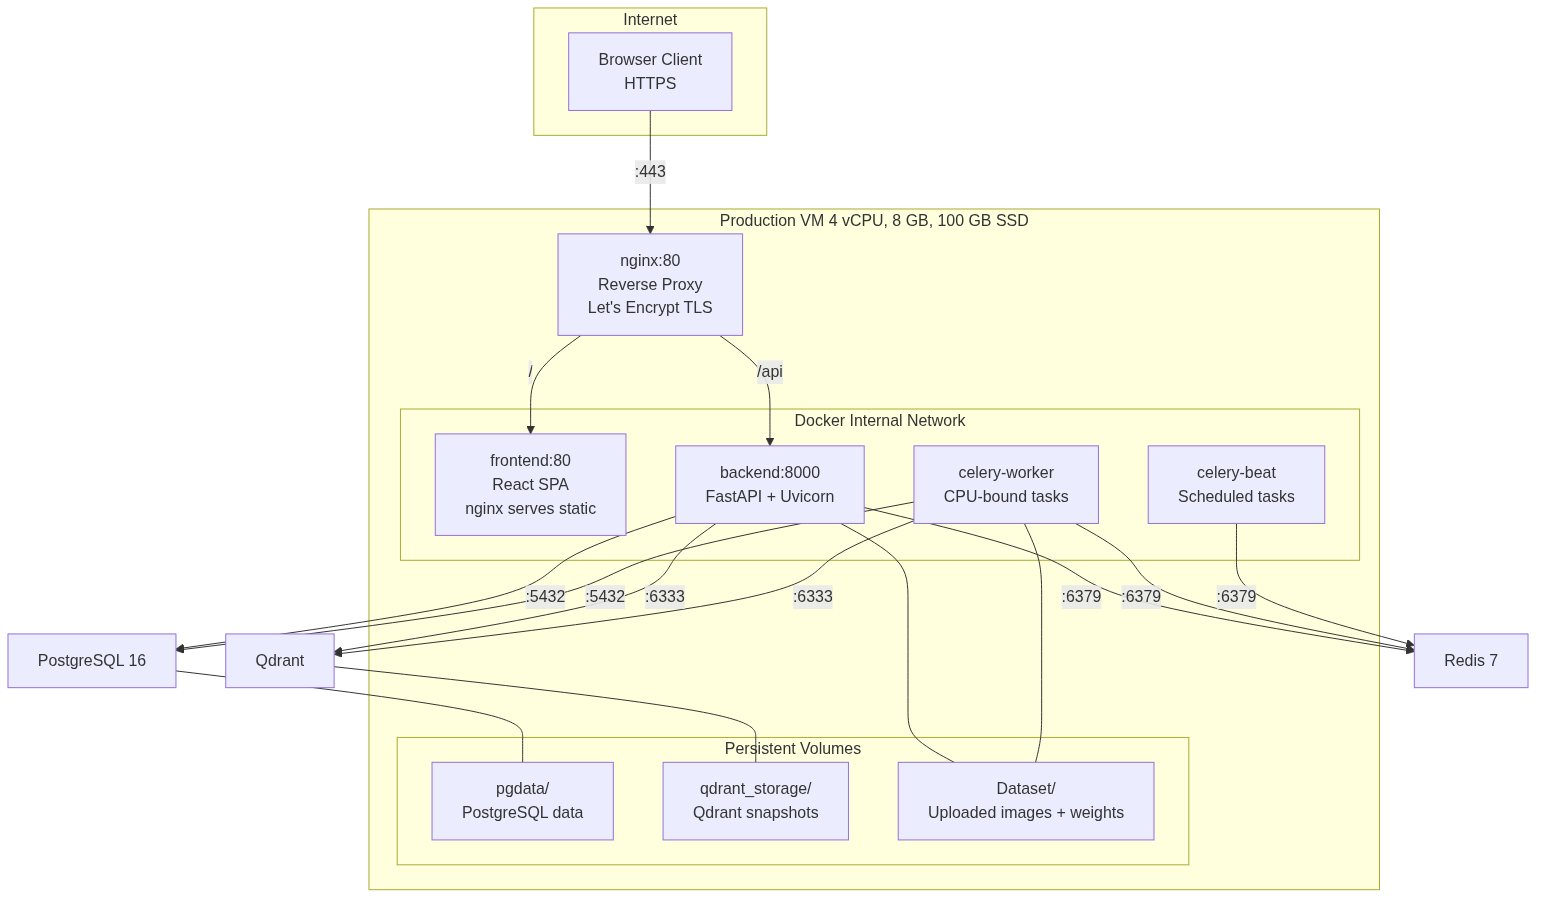
\includegraphics[width=\textwidth,height=0.65\textheight,keepaspectratio]{ch03_deployment.png}
    \end{column}
    \begin{column}{0.48\textwidth}
      \textbf{Docker Compose:}
      \begin{itemize}
        \item 6 services, internal network
        \item Persistent volumes (DB, uploads, Qdrant)
        \item Nginx reverse proxy
      \end{itemize}

      \textbf{CI/CD (GitHub Actions):}
      \begin{itemize}
        \item Backend: ruff $\rightarrow$ mypy $\rightarrow$ pytest
        \item Frontend: ESLint $\rightarrow$ tsc $\rightarrow$ build
        \item Manual deploy after PR merge
      \end{itemize}
    \end{column}
  \end{columns}
\end{frame}

% ===== SECTION: AGENTIC ENGINEERING =====
\section{Agentic Engineering}

% ===== SLIDE 26: AUTOLAB =====
\begin{frame}{Autolab -- 5-Agent Orchestration}
  \begin{center}
    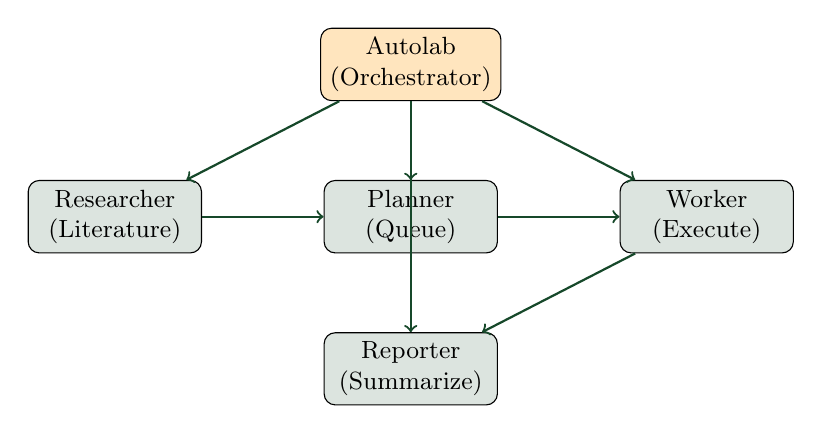
\begin{tikzpicture}[
      box/.style={draw, rounded corners, minimum width=2.2cm, minimum height=0.9cm, align=center, font=\small},
      arrow/.style={->, thick, mycoDark}
    ]
      \node[box,fill=mycoAccent!30] (orch) {Autolab\\(Orchestrator)};
      \node[box,below left=1cm and 1.5cm of orch,fill=mycoDark!15] (res) {Researcher\\(Literature)};
      \node[box,below=1cm of orch,fill=mycoDark!15] (plan) {Planner\\(Queue)};
      \node[box,below right=1cm and 1.5cm of orch,fill=mycoDark!15] (work) {Worker\\(Execute)};
      \node[box,below=1cm of plan,fill=mycoDark!15] (rep) {Reporter\\(Summarize)};
      \draw[arrow] (orch) -- (res);
      \draw[arrow] (orch) -- (plan);
      \draw[arrow] (orch) -- (work);
      \draw[arrow] (orch) -- (rep);
      \draw[arrow] (res) -- (plan);
      \draw[arrow] (plan) -- (work);
      \draw[arrow] (work) -- (rep);
    \end{tikzpicture}
  \end{center}
  \vspace{0.3em}
  \textbf{Worker isolation:} git worktrees under \texttt{.runtime/worktrees/}. Max 2 concurrent. Removed after run, best retained until merged.
\end{frame}

% ===== SLIDE 27: AGENT ROLES =====
\begin{frame}{Agent Roles}
  \begin{table}
    \centering
    \begin{tabular}{@{}llp{5cm}@{}}
      \toprule
      \textbf{Agent} & \textbf{Model} & \textbf{Responsibility} \\
      \midrule
      \rowcolor{mycoAccent!15}
      Autolab & BigBrain & Orchestrator -- delegates to all subagents \\
      Researcher & BigBrain & Literature scout: web/PDF $\rightarrow$ hypotheses \\
      Planner & MidBrain & Queue coordinator: assigns run\_ids \\
      Worker & MiniBrain & Isolated runner: worktree, execute, log \\
      Reporter & MiniBrain & Status summarizer: CSV $\rightarrow$ F1 summary \\
      \bottomrule
    \end{tabular}
  \end{table}

  \textbf{Hypothesis pipeline:} Researcher proposes $\rightarrow$ Planner validates duplicates $\rightarrow$ Worker tests in isolation $\rightarrow$ Reporter logs best F1
\end{frame}

% ===== SLIDE 28: GUARDRAILS =====
\begin{frame}{Guardrails \& Context Management}
  \begin{columns}[T]
    \begin{column}{0.5\textwidth}
      \textbf{Reducing Hallucinations:}
      \begin{enumerate}
        \item \textbf{SDD (Spec-Driven)}
        \begin{itemize}
          \item Living Spec, speckit toolchain
          \item Drift detection and resolution
        \end{itemize}
        \vspace{0.3em}
        \item \textbf{TDD (Test-Driven)}
        \begin{itemize}
          \item Failing test $\rightarrow$ fix $\rightarrow$ verify
          \item Every change has evidence
        \end{itemize}
        \vspace{0.3em}
        \item \textbf{Specialized Skills}
        \begin{itemize}
          \item Bounded instructions (react-best-practices, fastapi)
        \end{itemize}
      \end{enumerate}
    \end{column}
    \begin{column}{0.5\textwidth}
      \textbf{Context Management:}
      \begin{enumerate}
        \item \textbf{Caveman Mode}
        \begin{itemize}
          \item $\sim$75\% token reduction
          \item Technical substance intact
        \end{itemize}
        \vspace{0.3em}
        \item \textbf{Subagents + Worktrees}
        \begin{itemize}
          \item Isolated per task
          \item Only relevant context loaded
        \end{itemize}
        \vspace{0.3em}
        \item \textbf{Reusable Skills}
        \begin{itemize}
          \item Encode workflows as skills
          \item Constrain to validated patterns
        \end{itemize}
      \end{enumerate}
    \end{column}
  \end{columns}
\end{frame}

% ===== SECTION: CONCLUSION =====
\section{Conclusion}

% ===== SLIDE 29: SUMMARY =====
\begin{frame}{Summary \& Future Work}
  \begin{columns}[T]
    \begin{column}{0.5\textwidth}
      \textbf{Achievements:}
      \begin{itemize}
        \item Retrieval: \textbf{83.3\%} on 8 \textit{Penicillium} species
        \item Web app: 11 pages, 47 endpoints, 14 tables
        \item 5-agent autonomous experiment system
        \item Open-set, modular, interpretable
        \item 13 feature extractors, 3 segmentation methods
      \end{itemize}
    \end{column}
    \begin{column}{0.5\textwidth}
      \textbf{Future:}
      \begin{itemize}
        \item Interactive seg $\rightarrow$ auto-finetune YOLO
        \item One-click in-app model training
        \item Batch processing, plate-level analysis
        \item Medium-aware ensemble weighting
        \item Integration with MycoBank / Index Fungorum
      \end{itemize}
      \begin{block}{Core Philosophy}
        AI not only as the product -- but as the primary driver of the development process.
      \end{block}
    \end{column}
  \end{columns}
\end{frame}

% ===== SLIDE 30: THANK YOU =====
\begin{frame}[plain]
  \vfill
  \centering
  {\Huge\textcolor{mycoDark}{\textbf{Thank You}}}

  \vspace{1em}
  {\Large Questions?}

  \vspace{2em}
  {\small MycoAI Retrieval -- Graduation Thesis, June 2025}

  \vspace{1em}
  {\footnotesize Advisors: Dr. Oanh Nguyen (HUST) \quad$\bullet$\quad Prof. Duong Vu (Utrecht)}
  \vfill
\end{frame}

\end{document}
